\section{n-gram language model}
The $n$-gram language model analyzes a sequence of symbols by examining sets of frames, known as $n$-grams. This model is designed to construct a natural language model based on the assumption that each new symbol is statistically influenced by the preceding symbols. For example, the phrase '\texttt{I am playing }' could be followed by '\texttt{a piano}' or '\texttt{with a dog}'. The $n$-gram model assumes that the continuation of this phrase depends solely on a finite window of preceding words or characters, and assigns '\texttt{a piano}' a certain probability of being the most natural continuation. However, as language modeling techniques have advanced, the $n$-gram model has largely been replaced by more sophisticated models, such as transformers\footnote{For more information on transformers, see \url{https://en.wikipedia.org/wiki/Transformer_(deep_learning_architecture)}}.

\begin{figure}[ht]
	\centering
	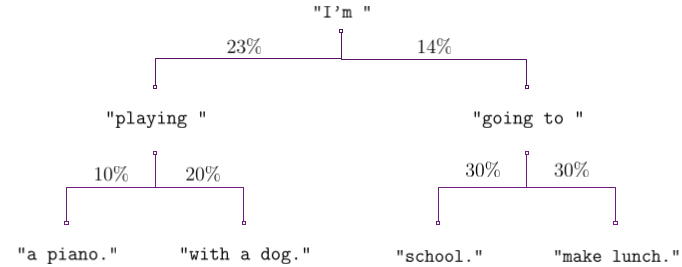
\includegraphics[width=\linewidth]{Figures/exngrammodel.png}
\end{figure}

\noindent The $n$-gram language model, first introduced by Shannon and described in \citet{Shannon_ngrammodel}, was later applied in \citet{SapAttribution} for the purpose of author attribution. In this case, the goal was not to generate natural text but to identify the author of a given text. The research found that the best performance was achieved using $8$-grams, and attribution was done by comparing each known author's work with the target text.

\noindent An additional development of this model extended its use to a completely different field: images. In the research thesis \cite{thesis}, this attribution method was employed to determine the authorship of a manuscript by treating the grams as square pixel tiles.

\subsection{Insights}
As previously mentioned, the $n$-gram model predicts the next characters or words to be placed based on the preceding ones. For example, if the focus is on sequences of $n$ printable characters, the model is trained on a dataset of text files, empirically deriving the probabilities $\mathbb{P}\left[w_n|w_1,\dots,w_{n-1}\right]$, where $w_i$ represents the $i$-th character of the $n$-gram.

\begin{toReview}
	\noindent In this way, a machine can construct a sentence from a few characters: $w_1,\ldots,w_{n-1}$. The algorithm iteratively selects the most probable next character $w_{n}$ given the current window of $n-1$ characters, then updates the window to $w_2,\ldots,w_{n}$ to predict $w_{n+1}$, and so on. This step-by-step process resembles a Markov chain, where each state corresponds to the current sequence of characters, and transitions between states occur with probabilities derived from the dataset.
\end{toReview}

\begin{modified}
\noindent The model assumes that the next character  depends only by the last $n-1$ characters so:
\begin{equation}
	\mathbb{P}\left[w_{n+k}|w_k\dots w_{n+k-1}\right] = \mathbb{P}\left[w_{n+k}|w_{k+1}\dots w_{n+k-1}\right] \quad \forall k
	\label{eq:ngram_model}
\end{equation}
\end{modified}
From this assumption we derive the following property:
\begin{proposition}
	\begin{modified}
		Let $w_1,\dots,w_{n-1},w_n\dots,w_{n+k}$ be a sequence of characters, where $n$ represents the size of the $n$-gram window used by the model. Specifically, the model assumes that the probability of the $n$-th character depends only on the preceding $n-1$ characters for all $n$-grams. We have that:
	\end{modified}
\begin{equation}
	\mathbb{P}\left[w_n,\dots,w_{n+k}|w_1,\dots,w_{n-1}\right] = \prod_{i=0}^{k}\mathbb{P}\left[w_{n+i}|w_{i+1}\dots w_{n+i-1}\right]
	\label{eq:ngram_model_prop}
\end{equation}
\end{proposition}

\begin{proof}
	This property is proved by using Bayes' theorem and the assumption of the model \cref{eq:ngram_model}:
\begin{align*}
	\mathbb{P}\left[w_n,\dots,w_{n+k}|w_1,\dots,w_{n-1}\right] &= \prod_{i=0}^{k}\mathbb{P}\left[w_{n+i}|w_1\dots w_{n+i-1}\right] \\
	&= \prod_{i=0}^{k}\mathbb{P}\left[w_{n+i}|w_{i+1}\dots w_{n+i-1}\right]
\end{align*}
\end{proof}

\noindent The model is built on the assumption that considering $n$-grams larger than $n$ is unnecessary. However, this limitation can introduce significant weaknesses in natural language processing, as it ignores information outside the $n$-character window. For instance, in a mystery novel, understanding the entire plot and its intricate details is crucial, something the model might overlook. Despite this, the $n$-gram model can still be quite effective in simpler contexts like everyday conversation. For example, after the input '\texttt{Hi! How are }', the model might predict '\texttt{you?}' as a natural continuation.

\noindent As mentioned earlier, this model was repurposed for a different goal by \citet{SapAttribution}. While the $n$-gram model might struggle to generate fully coherent natural language without encountering semantic inconsistencies or syntactic errors, it remains useful for capturing an author's writing style. This is achieved by training the model exclusively on texts by that author. The approach is to extract all $n$-grams from the target work and compare their distribution to that of known works by other authors. The proposed formula for comparing work $A$ with work $B$ is as follows:
\begin{equation}
	d(A,B) = \frac{1}{|D_A|+|D_B|}\sum_x\left(\frac{f_A(x)-f_B(x)}{f_A(x)+f_B(x)}\right)^2
	\label{eq:SapAttribution_dist}
\end{equation}
where $f_A(x)$ represents the frequency of the $n$-gram $x$ in the work $A$ and $|D_A|$ is the variety of observed $n$-grams.

\noindent As highlighted in \cite{thesis}, two relevant properties of this method of comparing distributions can be mentioned:
\begin{itemize}
	\item Each addendum of the summation takes on a value between $0$ and $1$.
	\item The external factor not only normalises the result so that it remains between $0$ and $1$, but also calls up the Jaccard index\footnote{For more about Jaccard index, see \url{https://en.wikipedia.org/wiki/Jaccard_index}}, improving the arithmetic mean of the summation:
	\[
		\frac{1}{|D_A|+|D_B|} = (1+J_{D_A,D_B})^{-1}\frac{1}{|D_A\cup D_B|}
	\]
	\begin{toReview}
		\noindent where $J_{D_A,D_B} := \frac{\left|D_A\cap D_B\right|}{\left|D_A\cup D_B\right|}$.

		\noindent In this way, we can see the comparison formula as a product between two types of index:
		\[
			d(A,B)=(1+J_{D_A, D_B})^{-1} \times \frac{1}{\left|D_A\cup D_B\right|}\sum_{x\in D_A\cup D_B}\left(\frac{f_A(x)-f_B(x)}{f_A(x)+f_B(x)}\right)^2
		\]
	\end{toReview}
\end{itemize}

\subsection{Implications}
We conclude this section by discussing the implications of this theory. As seen in \cref{eq:ngram_model}, no distinction is made between one $n$-gram and another. This is because $n$-grams of length 3, or slightly longer, are typically used, which are insufficient to cover a full word. However, when using $7$-grams, it becomes possible to consider the relationships between synonyms and distances between $n$-grams. For instance, we would expect some level of correlation between ‘\texttt{paper}’ and ‘\texttt{article}’ as they are synonyms.

\noindent In written texts, this rarely impacts the outcome, as there are relatively few synonyms for each term within the full vocabulary, and especially few long chains of synonyms. For example, it is unlikely that many synonyms for ‘\texttt{paper}’ begin with the string ‘\texttt{p}’ or ‘\texttt{pe}’.

\noindent As noted in \cite{thesis}, the research deliberately set appropriate image \textit{resolution} and \textit{posterization} to avoid discussions about the similarity between tiles. By controlling these parameters, the focus remained on the attribution process rather than getting lost in complex considerations of tile ‘synonyms’ and their potential concatenations.

\bigskip
We further examine the properties of the comparison formula defined in  \cref{eq:SapAttribution_dist}, particularly focusing on the problem of sparsity in $n$-grams.

\noindent Let $N$ represent the samples drawn from two absolutely continuous distributions $\mathcal{A}$ and $\mathcal{B}$ defined on $\mathbb{R}$. We partition $\mathbb{R}$ into intervals (boxes) of amplitude $1 \; / \; C$, thus transforming the original distributions into their discretized versions, $\mathcal{A}(C)$ and $\mathcal{B}(C)$, along with their respective samples.

\begin{figure}[ht]
	\centering
	\begin{subfigure}{0.45\linewidth}
		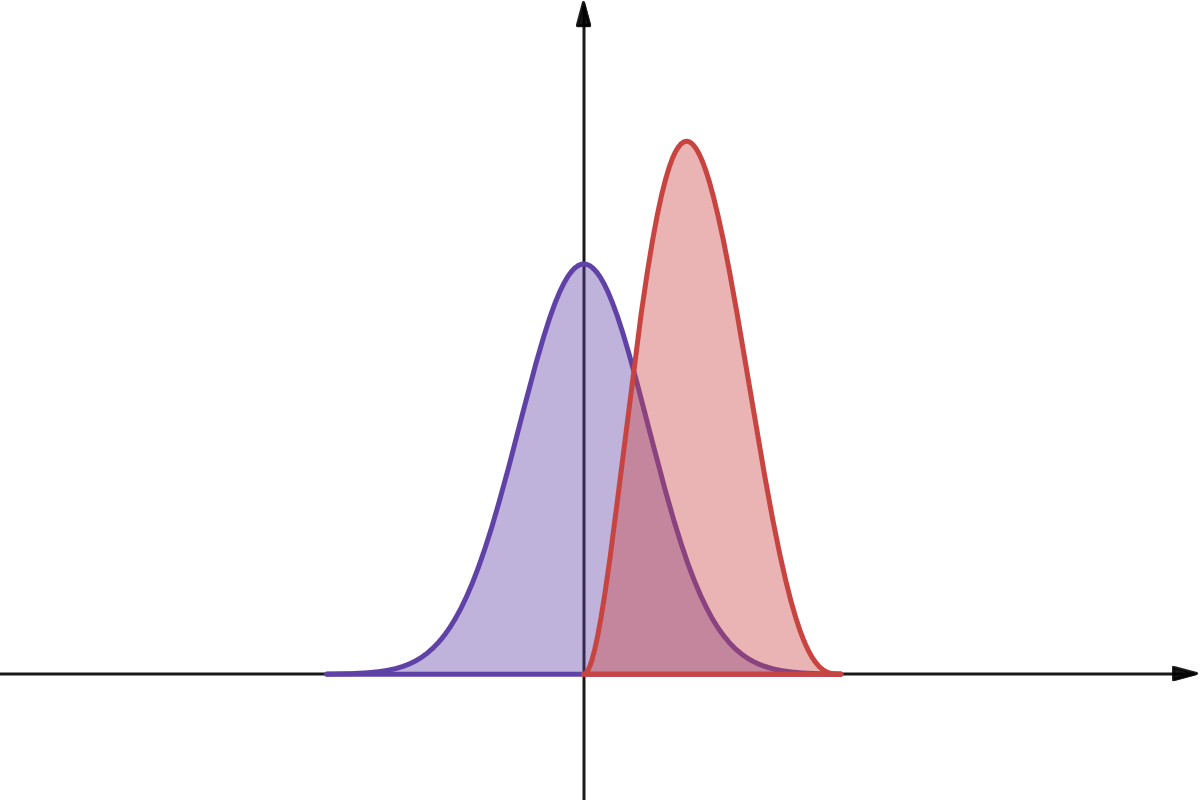
\includegraphics[width=\linewidth]{Figures/exnmodel_AB_cont.png}
	\end{subfigure} \begin{subfigure}{0.45\linewidth}
		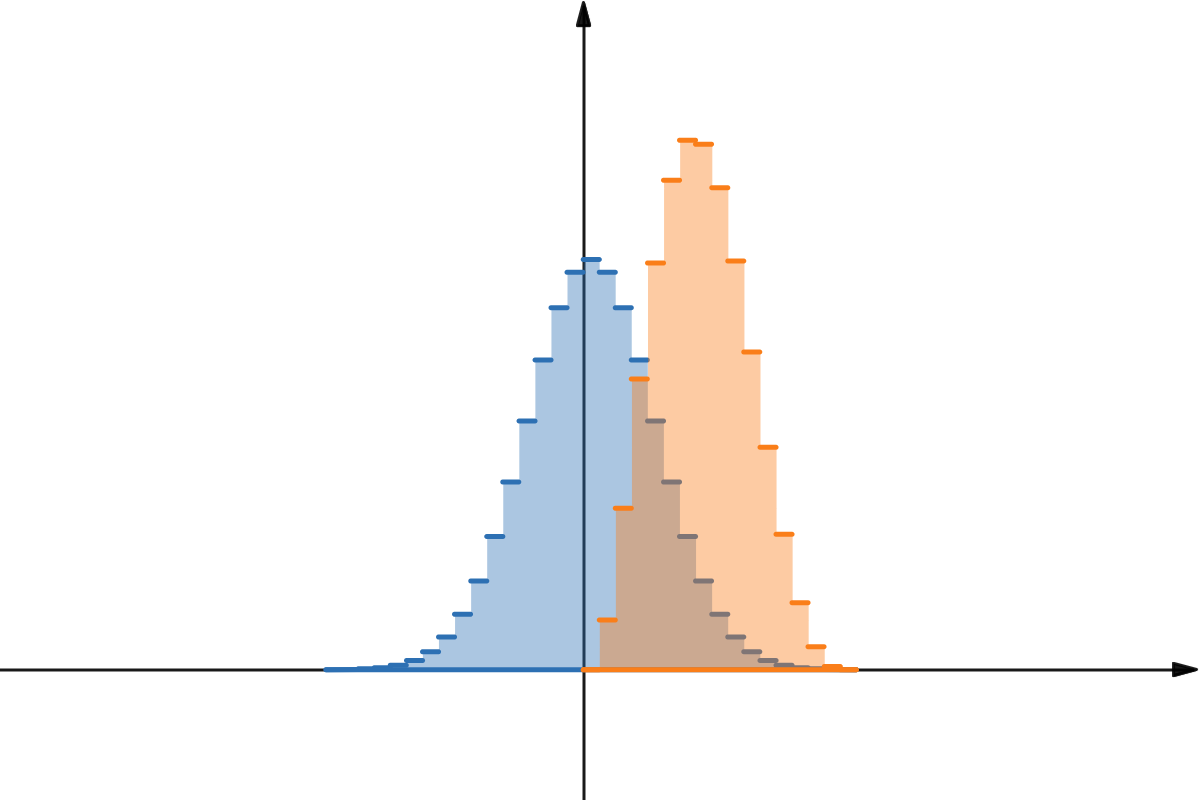
\includegraphics[width=\linewidth]{Figures/exnmodel_AB_disc.png}
	\end{subfigure}
\end{figure}

\noindent Now, let’s consider \cref{eq:SapAttribution_dist} and analyze the behavior of the estimated distance as the number of data points and the size of the boxes vary. By fixing the number of data points and decreasing the size of the boxes, the estimated distance gradually approaches $1$. This phenomenon occurs because there exists a critical dimension for $1 \;/ \; C$, such that with a sufficiently high probability, each sample becomes isolated within its own box. Consequently, this drives $J_{D_A,D_B}$ toward $0$, making each term in the summation equal to $1$.

\bigskip
In \cite{thesis}, the continuous nature of the $n$-tiles was addressed by discretizing the continuous space in which they were defined, fixing a resolution and applying posterization.\begin{toReview} Posterization is a process that reduces the number of discrete levels of color or intensity in an image, effectively mapping a continuous range of values into a smaller set of intervals. For example, in a color image, subtle variations in shades of red might all be grouped into a single pure red, removing the nuance of intermediate shades. \end{toReview} However, this approach results in a significant loss of information. Therefore, this paper will explore a method to achieve a cleaner and more dynamic discretization.
